% !TeX spellcheck = en_US
% !TEX TS-program = pdflatex
% !TEX encoding = IsoLatin

%% Version 4x3 und 16x9  2.2 02.01.2014

%Based on ETH official latex template
%Modified for ASL by Alvaro Estandia (09.02.2015) (ealvaro@student.ethz.ch)

% ==== wrapper class ==========================================================
\documentclass[% wrapper-class ETHpres option inspite of aspectratio for beamer-classe
    fourtothree=true, % true (default) -- 4:3-format, false -- 16:9-format
    DepLogo=true     % true -- use deplogo_13.pdf, false (default) 
                      %         do not use deplogo_13.pdf for footer
    ]{ETHpres}

% ==== misc: you may use or not ===============================================
%\usepackage{graphicx}   % for including figures
%%\graphicspath{{pictures/}}
%\usepackage{tabularx}   % for special table environment (tabularx-table)
%\usepackage{booktabs}   % for table layout
%\usepackage{natbib}     % for bibliography with astron-style
%\bibliographystyle{astron}
%\usepackage{siunitx}    % to use for international units in the real world
%\usepackage[
%    colorlinks=true, linkcolor=white, urlcolor=white, % this is special for this presentation here to get the toc in white
%    hypertexnames=false,% for correct links (duplicate-error solution)
%	setpagesize=false,  % necessary in order to not change text-/paperformat for the document
%	pdfborder={0 0 0},  % removes border around links
%	pdfpagemode=FullScreen,% open pdf in full screen mode
%    pdfstartview=Fit    % fit page to pdf viewer
%]{hyperref}% all links stay black and are thus invisible

%----- My Packages
\titlespacing{\section}{0pt}{-25pt}{0pt}
\titlespacing{\subsubsection}{0pt}{5pt}{0pt}

\usepackage{amsmath}
\usepackage{caption}
\usepackage{comment}
\usepackage[makeroom]{cancel}


\setitemize{noitemsep,topsep=0pt,parsep=0pt,partopsep=0pt}

%\usepackage{soul} Highligh text \hl{Some Text}
\usepackage{media9} %Add videos

%ASL Packages
\usepackage[numbers]{natbib}
\usepackage{enumitem}
\usepackage{units}

\usepackage{isomath}
\renewcommand{\vec}{\vectorsym}
\newcommand{\mat}{\matrixsym}


% ==== language ================================================================
\usepackage[latin1]{inputenc}
%\usepackage[utf8]{inputenc}
% English
\usepackage[english]{babel}
\AtBeginDocument{\renewcaptionname{english}{\contentsname}{ }}% toc-name
%% Deutsch
%\usepackage[ngerman]{babel}
%\AtBeginDocument{\renewcaptionname{ngerman}{\contentsname}{ }}% toc-name

% ==== choose the basic color for your presentation ===========================
% colorbar-color
\colorlet{firstcolor}{ETHc} % see pages 2  and 3 of this sample presentation
% bachground color titlepage
\colorlet{secondcolor}{ETHc} % see pages 2  and 3 of this sample presentation

% === fill in first information for the presentation ==========================
\newcommand*{\ETHtitle}{TITLE}
\newcommand*{\ETHauthor}{AUTHOR}
\newcommand*{\ETHdate}{DATE}


\begin{document}
% =========== begin of titlepage ============
\ETHtitelbild\textcolor{white}{\large\textbf{\ETHtitle}}\\~\newline\hspace{6mm}\normalsize%
%%
% ==== start here with the text on the titlepage
\textcolor{white}{
\textbf{\ETHauthor}\\ \\
TYPE OF PROJECT\\
Supervised by }\\
%%

\clearpage
% =========== begin of the standard page ============

\ETHslide
\section*{Overview}
\tableofcontents

\clearpage

\ETHslide
\section*{Adding a video}
\addcontentsline{toc}{section}{Adding a video}
%Example included because it took me very long to figure it out.
\includemedia[
		  width=0.8\textwidth,
		  height=0.45\textwidth,
		  activate=pageopen,
		  addresource=LittleDog.mp4,
		  flashvars={source=LittleDog.mp4}
		]{}{VPlayer.swf}\\
		\footnotesize{LittleDog walking over rough terrain (S. Schaal, ``The latest version of the LittleDog Robot,'' 2010. https://www.youtube.com/watch?v=nUQsRPJ1dYw)}
			
\clearpage


\ETHslide
\section*{Adding a video - Example Slide}
\addcontentsline{toc}{subsection}{Example Slide}
\begin{minipage}{0.6\textwidth}
	\begin{itemize}
		\item[\ETHitem] Point 1
		\item[\ETHitem] Point 2
		\begin{itemize}
			\item Point 1.1
			\item Point 1.2
		\end{itemize}
\end{itemize}
\end{minipage}
\begin{minipage}{0.39\textwidth}
	\centering
	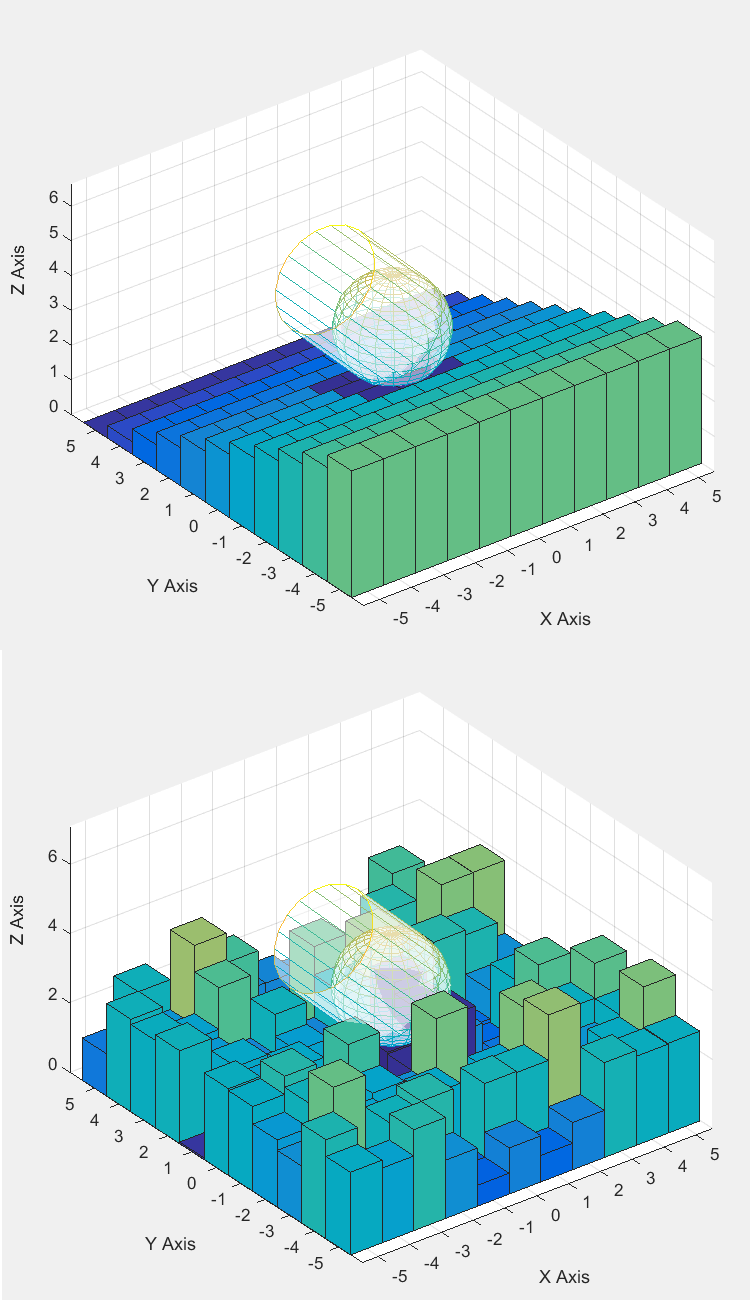
\includegraphics[width=0.75\textwidth]{SlopeStdDev.png}\\
	\footnotesize{Caption}
\end{minipage}

\begin{comment}
	Add a video file
	
	\includemedia[
	 width=\textwidth,
	 height=0.55\textwidth,
	 activate=pageopen,
	 addresource=Video/BigDog.mp4,
	 flashvars={source=Video/BigDog.mp4}
			]{}{VPlayer.swf}
	\footnotesize{Caption}
	
	\end{comment}

\clearpage

\begin{comment}
References Slide
\ETHslide
\addcontentsline{toc}{section}{References}
\bibliographystyle{bibliography/IEEEtranN}
\tiny{
\bibliography{FILE}}
\clearpage
\end{comment}
\end{document}


